\documentclass[11pt]{article}
\usepackage[toc,page]{appendix}
\usepackage{amsmath, amssymb}
\usepackage[utf8]{inputenc}
\usepackage[T1]{fontenc}
\usepackage[style=apa,backend=biber]{biblatex}
%\usepackage{biblatex}
\addbibresource{references.bib}
\usepackage{graphicx}
\usepackage{tikz}
\usetikzlibrary{automata,positioning,shapes.geometric, arrows.meta, fit, backgrounds, calc, chains}
\graphicspath{./images/Easy_Pictures/SAR_ADD_Rounding}%\usepackage{kpfonts}
\usepackage{float}
\usepackage[margin=1in]{geometry}
\usepackage{cancel}
\usepackage{epsfig}
\usepackage{tikz-3dplot}
\usepackage{darkmode}
\usepackage{dirtytalk}
\usepackage{longtable,booktabs,array}
\usepackage{calc} % for calculating minipage widths
\usepackage[utf8]{inputenc}
\usepackage[T1]{fontenc}
\usepackage{xcolor}
\usepackage{listings}


\usepackage{etoolbox}
\usepackage{hyperref}
\hypersetup{
    colorlinks=true,
    linkcolor=blue,
    filecolor=magenta,      
    urlcolor=cyan,
    pdftitle={Hermeneutic Calculator},
    citecolor=blue,
    }


\urlstyle{same}

\lstdefinestyle{htmlStyle}{
    language=HTML,
    basicstyle=\ttfamily\small,
    keywordstyle=\color{blue}\bfseries,
    commentstyle=\color{gray}\itshape,
    stringstyle=\color{red},
    breaklines=true,
    frame=single,
    numbers=left,
    numberstyle=\tiny\color{gray},
    columns=fullflexible,
}
\lstdefinelanguage{HTML}{
  keywords={<!DOCTYPE, html, head, title, body, h1, h2, h3, p, div, span, a, img, ul, li, table, tr, td, th, style, link, script},
  sensitive=true,
  comment=[l]{//},
  morecomment=[s]{/*}{*/},
  morestring=[b]',
  morestring=[b]"
}
\lstset{style=htmlstyle, language=html}
% Updated to explicitly pass the language option
%\lstinputlisting[style=htmlstyle, language=html]{./html/example.html}
%\usepackage{tocloft}

% Optional: define some custom colors
\definecolor{sliceRed}{RGB}{225,224,91} % matching "varyellow" from your code
\definecolor{linkYellow}{RGB}{255,215,0}  % a golden yellow
\tdplotsetmaincoords{70}{110}

\title{Addition Strategies: Rounding and Adjusting}
\author{Compiled by: Theodore M. Savich}



\begin{document}
\maketitle

\subsection*{Transcript}
Video from \textcite{Carpenter1999}. Strategy descriptions and examples adapted from \textcite{HackenbergCourseNotes}. 
\begin{itemize}
\item \textbf{Teacher:} Lucy has eight fish. She wants to buy five more fish. How many fish will Lucy have then?
 

\item \textbf{Robert:} 13 

\item \textbf{Teacher:} How'd you get the 13?

\item \textbf{Robert:} I just took the eight out. And then I, if she had ten fish, it would have been 15. If she had nine fish, it would have been 14. And if it would have been eight fish, which it was, it would have been 13. So, I just got 13. 

\item \textbf{Teacher:} Did you use those blocks to solve this problem?

\item \textbf{Robert:} Well, I only used eight. I didn't use the other five, though. I used part of it in here (gestures to the mat with the blocks) and part of it in my head. you get 13.
\end{itemize}

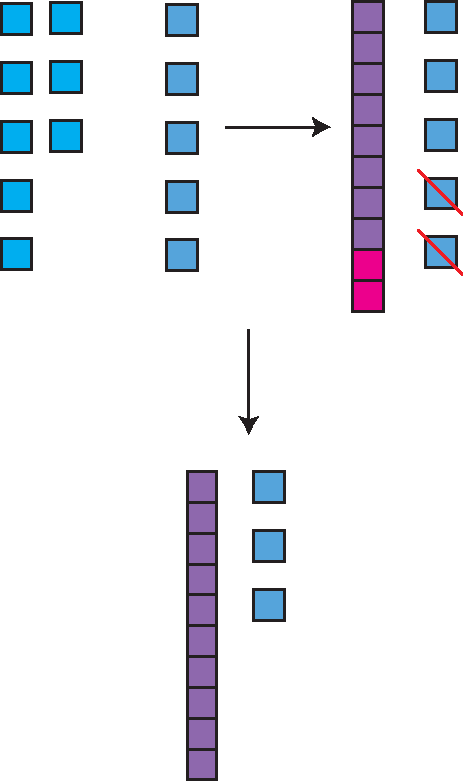
\includegraphics[width=.25\textwidth]{images/Easy_Pictures/SAR_ADD_Rounding/PDF/SAR_ADD_Rounding.pdf}

\noindent \textbf{Notation Representing Robert's Solution:}

\begin{align*}
8 + 5 &= \Box \\
8+2 &= 10\\
10+5 &= 15\\
8+5 &= 15-2\\
8+5 &= 13\\
\end{align*}

\subsubsection*{Description of Strategy:}

 \textbf{Objective:} Rounding for Simplicity:
 We start by changing at least one number to a ``friendlier'' value --- usually rounding it to the closest whole number of bases. For instance, if a number is just a few ones short of a multiple of 10, we can round it up so that it becomes exactly that multiple. This makes the arithmetic easier because we have well-known patterns (adding a full group of 10, for example) where the ones digit remains unchanged and only the tens (or ``base'') digit increases.
 
 \begin{enumerate}
 \item \textbf{The Need to Adjust:} When you round up a number, you are effectively adding a little extra to it. As a result, when you solve the simplified problem, your computed sum is slightly too high compared to the original one. To correct for this, you must subtract the extra amount that you added. Conversely, if you had rounded down (i.e., subtracted some value to simplify the number), then your computed sum would be too low, and you would need to add that amount back in.
 \item \textbf{Why the Inverse Operation?} The principle is simple: whatever operation you use to alter the number for ease of calculation must be undone by the inverse operation to return to the original value.
 \begin{itemize}\item If you \textbf{add} to round a number up, you must \textbf{subtract} later to adjust.
 \item If you \textbf{subtract} to round a number down, you must \textbf{add} back the same amount after solving.
 \end{itemize}
 This two-step process—first simplifying via rounding and then adjusting—helps you manage complex addition while keeping the final answer accurate to the original numbers.
\end{enumerate}
 
 
 
 
 
 

\subsection*{Rounding and Adjusting}

\subsubsection*{Description of Strategy}

\begin{itemize}
    \item \textbf{Objective:} Round one addend to a convenient number (usually a base multiple), perform the addition, then adjust the result.
    \item \textbf{Example:} $46 + 37$
    \begin{itemize}
        \item Round $46$ up to $50$ (adding $4$).
        \item Add: $50 + 37 = 87$.
        \item Adjust: Subtract the $4$ added earlier: $87 - 4 = 83$.
    \end{itemize}
\end{itemize}

\subsubsection*{Automaton Type}
\textbf{Pushdown Automaton (PDA)}: Needed to remember the adjustment amount.

\subsubsection*{Corrected Automaton (Register Machine Model)}

We define a Register Machine that models "Rounding and Adjusting" as an elaboration that utilizes previously learned strategies as cognitive subroutines. This model assumes the "Round Up, Adjust Down" variant.

\textbf{M = (Q, V, \delta, q_0, F)}

\begin{itemize}
    \item \textbf{States (Q):} {$q_{start}, q_{calc\_K}, q_{add}, q_{adjust}, q_{accept}$}
    \item \textbf{Registers (V):} {Target (Number to round), Other (Second addend), K (Adjustment), A\_rounded, TempSum, Result}
\end{itemize}

\textbf{Transition Function (\delta) - Highlighting Elaboration:}

\begin{longtable}{|l|l|l|l|}
\hline
\textbf{Current State} & \textbf{Next State} & \textbf{Subroutine/Action} & \textbf{Interpretation} \\
\hline
\endhead
$q_{start}$ & $q_{calc\_K}$ & Read A, B. (Heuristic: Select Target/Other) & Start. Select number closer to the next base. \\
\hline
$q_{calc\_K}$ & $q_{add}$ & \textbf{Count Up To Base(Target)} -> K, A\_rounded & Determine K by counting up from Target to the next base. \\
\hline
$q_{add}$ & $q_{adjust}$ & \textbf{COBO(A\_rounded, Other)} -> TempSum & Add Other to the rounded A. (Efficient as A\_rounded is a base). \\
\hline
$q_{adjust}$ & $q_{accept}$ & \textbf{Count Back(TempSum, K)} -> Result & Adjust by counting back K from the TempSum. \\
\hline
\end{longtable}

\subsubsection*{Automaton Diagram for Rounding and Adjusting}

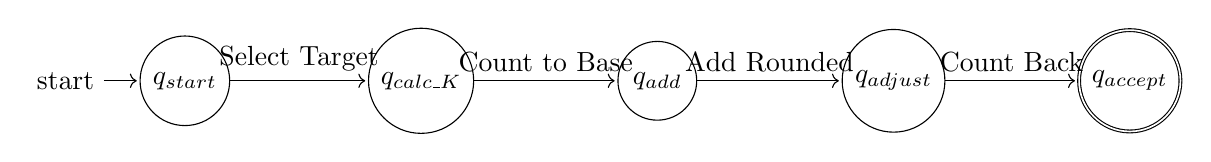
\begin{tikzpicture}[
    shorten >=1pt,
    node distance=3cm,
    on grid,
    auto,
    every state/.style={minimum size=1cm, align=center}
]
    % States
    \node[state, initial] (start) {$q_{start}$};
    \node[state, right=of start] (calc_k) {$q_{calc\_K}$};
    \node[state, right=of calc_k] (add) {$q_{add}$};
    \node[state, right=of add] (adjust) {$q_{adjust}$};
    \node[state, accepting, right=of adjust] (accept) {$q_{accept}$};
    
    % Transitions
    \path[->]
        (start) edge node {Select Target} (calc_k)
        (calc_k) edge node {Count to Base} (add)
        (add) edge node {Add Rounded} (adjust)
        (adjust) edge node {Count Back} (accept);
\end{tikzpicture}

\subsubsection*{Python Implementation}

\begin{lstlisting}[language=Python]
import pandas as pd

class RoundingAdjustingAutomaton:
    """
    A Register Machine model simulating the 'Rounding and Adjusting' strategy.
    This model is elaborated by utilizing 'Counting Up To', 'COBO' (for addition
    with bases), and 'Counting Back' (for adjustment) as internal iterative processes.
    """
    def __init__(self, A, B, Base=10):
        self.A_initial = A
        self.B_initial = B
        self.Base = Base

        # Heuristic: Apply the strategy to the number closer to the next base.
        # We check which number has the largest remainder (if not 0).
        A_rem = A % Base if A != 0 else 0
        B_rem = B % Base if B != 0 else 0

        if A_rem >= B_rem:
            self.Target = A
            self.Other = B
        else:
            self.Target = B
            self.Other = A

        # Registers
        self.K = 0
        self.A_rounded = 0
        self.TempSum = 0
        self.Result = 0

        # Internal registers for iterative processes (subroutines)
        self.internal_counter = 0
        self.internal_value = 0

        self.state = 'q_start'
        self.history = []

    def _record_history(self, interpretation, highlight=False):
        self.history.append({
            'State': self.state, 'Interpretation': interpretation,
            'K': self.K, 'A_rounded': self.A_rounded, 'TempSum': self.TempSum, 'Result': self.Result,
            'Highlight': highlight
        })

    def transition(self, next_state):
        self.state = next_state
        # Reset internal counters when transitioning to a new phase
        self.internal_counter = 0
        self.internal_value = 0

    def run(self):
        while self.state not in ['q_accept', 'q_error']:
            if self.state == 'q_start':
                self.execute_start()
            elif self.state == 'q_calc_K':
                self.execute_calc_K()
            elif self.state == 'q_add':
                self.execute_add()
            elif self.state == 'q_adjust':
                self.execute_adjust()
            else:
                self.transition('q_error')
                break
        return self.Result

    def execute_start(self):
        """q_start: Read inputs and determine rounding target."""
        self._record_history(f"Inputs: {self.A_initial}, {self.B_initial}. Target for rounding: {self.Target}", highlight=True)
        self.transition('q_calc_K')

    def execute_calc_K(self):
        """q_calc_K: Subroutine: Count Up To Base."""

        # Determine the target base
        if self.Target == 0:
             target_base = 0
        elif self.Target % self.Base == 0:
             target_base = self.Target
        else:
             target_base = ((self.Target // self.Base) + 1) * self.Base

        if self.internal_value == 0:
            # Initialize
            self.internal_value = self.Target
            self.K = 0

        if self.internal_value < target_base:
            # Iterative counting up
            self.internal_value += 1
            self.K += 1
            self._record_history(f"Counting Up: {self.internal_value}, K={self.K}")
        else:
            # Reached the base
            self.A_rounded = target_base
            self._record_history(f"K needed is {self.K}. Target rounded to {self.A_rounded}.", highlight=True)
            self.transition('q_add')

    def execute_add(self):
        """q_add: Subroutine: COBO(A_rounded, Other)."""

        if self.internal_counter == 0 and self.internal_value == 0:
            # Initialize COBO process
            self.TempSum = self.A_rounded
            # Decompose 'Other'
            self.internal_value = self.Other // self.Base # BaseCounter
            self.internal_counter = self.Other % self.Base # OneCounter

        # COBO Phase 1: Add Bases
        if self.internal_value > 0:
            self.TempSum += self.Base
            self.internal_value -= 1
            self._record_history(f"COBO (Base): {self.TempSum}")
            return

        # COBO Phase 2: Add Ones
        if self.internal_counter > 0:
            self.TempSum += 1
            self.internal_counter -= 1
            self._record_history(f"COBO (One): {self.TempSum}")
            return

        # COBO Complete
        self._record_history(f"{self.A_rounded} + {self.Other} = {self.TempSum}.", highlight=True)
        self.transition('q_adjust')

    def execute_adjust(self):
        """q_adjust: Subroutine: Count Back(TempSum, K)."""

        if self.internal_counter == 0:
             # Initialize Counting Back
             self.Result = self.TempSum
             self.internal_counter = self.K # Count down K times

        if self.internal_counter > 0:
            # Iterative counting back
            self.Result -= 1
            self.internal_counter -= 1
            self._record_history(f"Counting Back: {self.Result}")
        else:
            # Adjustment complete
            self._record_history(f"Subtracted K ({self.K}). Final Result: {self.Result}.", highlight=True)
            self.transition('q_accept')

    def display_history(self, summarized=True):
        print(f"\n--- Rounding and Adjusting Execution History ({self.A_initial} + {self.B_initial}) ---")
        df = pd.DataFrame(self.history)
        display_cols = ['State', 'Interpretation', 'K', 'A_rounded', 'TempSum', 'Result']

        if summarized:
             print("Summary Trace:")
             summary_df = df[df['Highlight'] == True]
             print(summary_df[display_cols].to_markdown(index=False))
        else:
            print("Full Iterative Trace:")
            print(df[display_cols].to_markdown(index=False))


# Test Case 1: Robert's example (8 + 5). Heuristic chooses 8.
ra_8_5 = RoundingAdjustingAutomaton(A=8, B=5)
ra_8_5.run()
ra_8_5.display_history(summarized=True)

# Test Case 2: 46 + 37. Heuristic chooses 37 (remainder 7 > remainder 6).
ra_46_37 = RoundingAdjustingAutomaton(A=46, B=37)
ra_46_37.run()
ra_46_37.display_history(summarized=False)
\end{lstlisting}

\subsubsection*{Execution Trace (46 + 37 - Full Iterative Trace):}
\begin{verbatim}
--- Rounding and Adjusting Execution History (46 + 37) ---
Full Iterative Trace:
| State      | Interpretation                                            |   K |   A_rounded |   TempSum |   Result |
|:-----------|:----------------------------------------------------------|----:|------------:|----------:|---------:|
| q_start    | Inputs: 46, 37. Target for rounding: 37                   |   0 |           0 |         0 |        0 |
| q_calc_K   | Counting Up: 38, K=1                                      |   1 |           0 |         0 |        0 |
| q_calc_K   | Counting Up: 39, K=2                                      |   2 |           0 |         0 |        0 |
| q_calc_K   | Counting Up: 40, K=3                                      |   3 |           0 |         0 |        0 |
| q_calc_K   | K needed is 3. Target rounded to 40.                      |   3 |          40 |         0 |        0 |
| q_add      | COBO (Base): 50                                           |   3 |          40 |        50 |        0 |
| q_add      | COBO (Base): 60                                           |   3 |          40 |        60 |        0 |
| q_add      | COBO (Base): 70                                           |   3 |          40 |        70 |        0 |
| q_add      | COBO (Base): 80                                           |   3 |          40 |        80 |        0 |
| q_add      | COBO (One): 81                                            |   3 |          40 |        81 |        0 |
| q_add      | COBO (One): 82                                            |   3 |          40 |        82 |        0 |
| q_add      | COBO (One): 83                                            |   3 |          40 |        83 |        0 |
| q_add      | COBO (One): 84                                            |   3 |          40 |        84 |        0 |
| q_add      | COBO (One): 85                                            |   3 |          40 |        85 |        0 |
| q_add      | COBO (One): 86                                            |   3 |          40 |        86 |        0 |
| q_add      | 40 + 46 = 86.                                             |   3 |          40 |        86 |        0 |
| q_adjust   | Counting Back: 85                                         |   3 |          40 |        86 |       85 |
| q_adjust   | Counting Back: 84                                         |   3 |          40 |        86 |       84 |
| q_adjust   | Counting Back: 83                                         |   3 |          40 |        86 |       83 |
| q_adjust   | Subtracted K (3). Final Result: 83.                       |   3 |          40 |        86 |       83 |
\end{verbatim}

\printbibliography
\end{document}